\chapter{NOGWs in ground-based Lidar observations}
% NOGWs 
% Lidar observations in Q3D simulations are not useful / used y position 1 instead on npy/2!! --> use local 2D simulations for analysis of these plots (eventually conduct constant wind simulation again

% interpretation
Observations of GWs in the upper atmosphere are sparse. AIRS on board of NASA’s Aqua satellite is presently the only instrument that provides temperature measurements for a limited altitude range applicable for the detection of GWs (e.g \cite[]{hindley_gravity_2019} or \cite[]{hindley_18year_2020}). Observations are available globally, but only on a daily basis and sensitive to just a portion of the gravity wave spectrum due to the so-called "observational filter" of the instrument properties (e.g. \cite[]{preusse_space-based_2002} or \cite[]{alexander_recent_2010}). Vertical temperature profiles from ground-based Lidar stations are currently the only alternative potentially available on a regular basis. They provide much higher vertical and temporal resolution on one hand, but in the end it is just a point observation limited to night-time and clear sky conditions. The analysis of GWs in these measurements is challenging and at a certain point not possible without consulting additional information from other observations or model data. 

High resolution vertical time series at multiple locations were retrieved from the idealized numerical simulations discussed in previous chapters, too. Though the proposed excitation mechanism of these NOGWs is supposed to mimic the excitation of MWs over topography, their potential appeareance in lidar observations would be different due to the propagation of their source. Therefore, section \ref{sec:lidOb-idealized} aims for a first analysis on how waves generated by propagating tropopause depressions would show up in vertical timeseries and how they could be interpreted. Subsequently, section \ref{sec:lidOb-coral} presents two measurements of the Compact Rayleigh Autonomous Lidar (CORAL) shortly described in chapter 2 that fit to the idealized simulations. A first interpretation based on ERA5 reanalysis data is discussed, but it can be anticipated that more effort in terms of a high resolution simulation would be needed to get to an explicit conclusion. 

\section{Lidar observations in idealized numerical simulations}
\label{sec:lidOb-idealized}
% The goal of the following analysis is

Wave properties of stationary mountain waves are somewhat unfavorable from a lidar observation point of view. Their horizontal phase speed vanishes ($c_{px}=0$) together with the ground-based frequency ($\omega$=0). As a result, phase lines in vertical time series of ground-based lidar observations appear horizontal and one can only derive the vertical wavelength $\lambda_z$ from the observations, but misses information on horizontal scales (e.g. \cite[]{dornbrack_interpretation_2017} or \cite[]{reichert_highcadence_2021}). Section \ref{sec:resultsQ3D} showed that NOGWs from a propagating source might develope similar properties, but within the reference frame moving with their source. Figure \ref{fig:lidar_sim} illustrates how this alters their appearance in vertical time series. As discussed in section \ref{sec:resultsQ3D}, the wave forcing of a trough moving with $c_{source}$ (\ref{fig:lidar_sim}b) for a certain point in time can be reproduced by a stationary trough with a wind profile reduced by $c_{source}$ (Figure \ref{fig:lidar_sim}c). However, phase lines in the vertical time series differ significantly and show an upward (downward) tilt for a source moving in the same (opposite) direction as the background wind (Figure \ref{fig:lidar_sim}d). Does this allow for a derivation of horizontal wave properties? Yes and no! Clearly, tilted phase lines enable the quantification of a ground-based period $T$ from the vertical time series, but linking this period to wave properties depends on the wave source and atmospheric background conditions. Multiple phenomena could explain upward tilted phase lines in lidar observations, so their intepretation requires additional knowledge on the prevailing processes and synoptic situation. Examples are:
%  so by considering lidar observations only, upward tilted phase lines could for example be attributed
% \cite[]{ern_absolute_2004}

\begin{itemize}
    \item downward propagating wave packets caused by reflection or wave breaking in the upper atmosphere which excites secondary waves that travel up and down from their source region (\cite[]{dornbrack_interpretation_2017} and \cite[]{vadas_mechanism_2003}).
    % fishbone pattern

    \item transient background conditions. Mainly in the form of a varying wind speed and wind direction.

    \item a GW source moving in the same direction as the background wind as illustreated in Figure \ref{fig:lidar_sim}d and \ref{fig:lidar_sim}f.
\end{itemize}

\begin{figure*}[tbp]
    \centering
    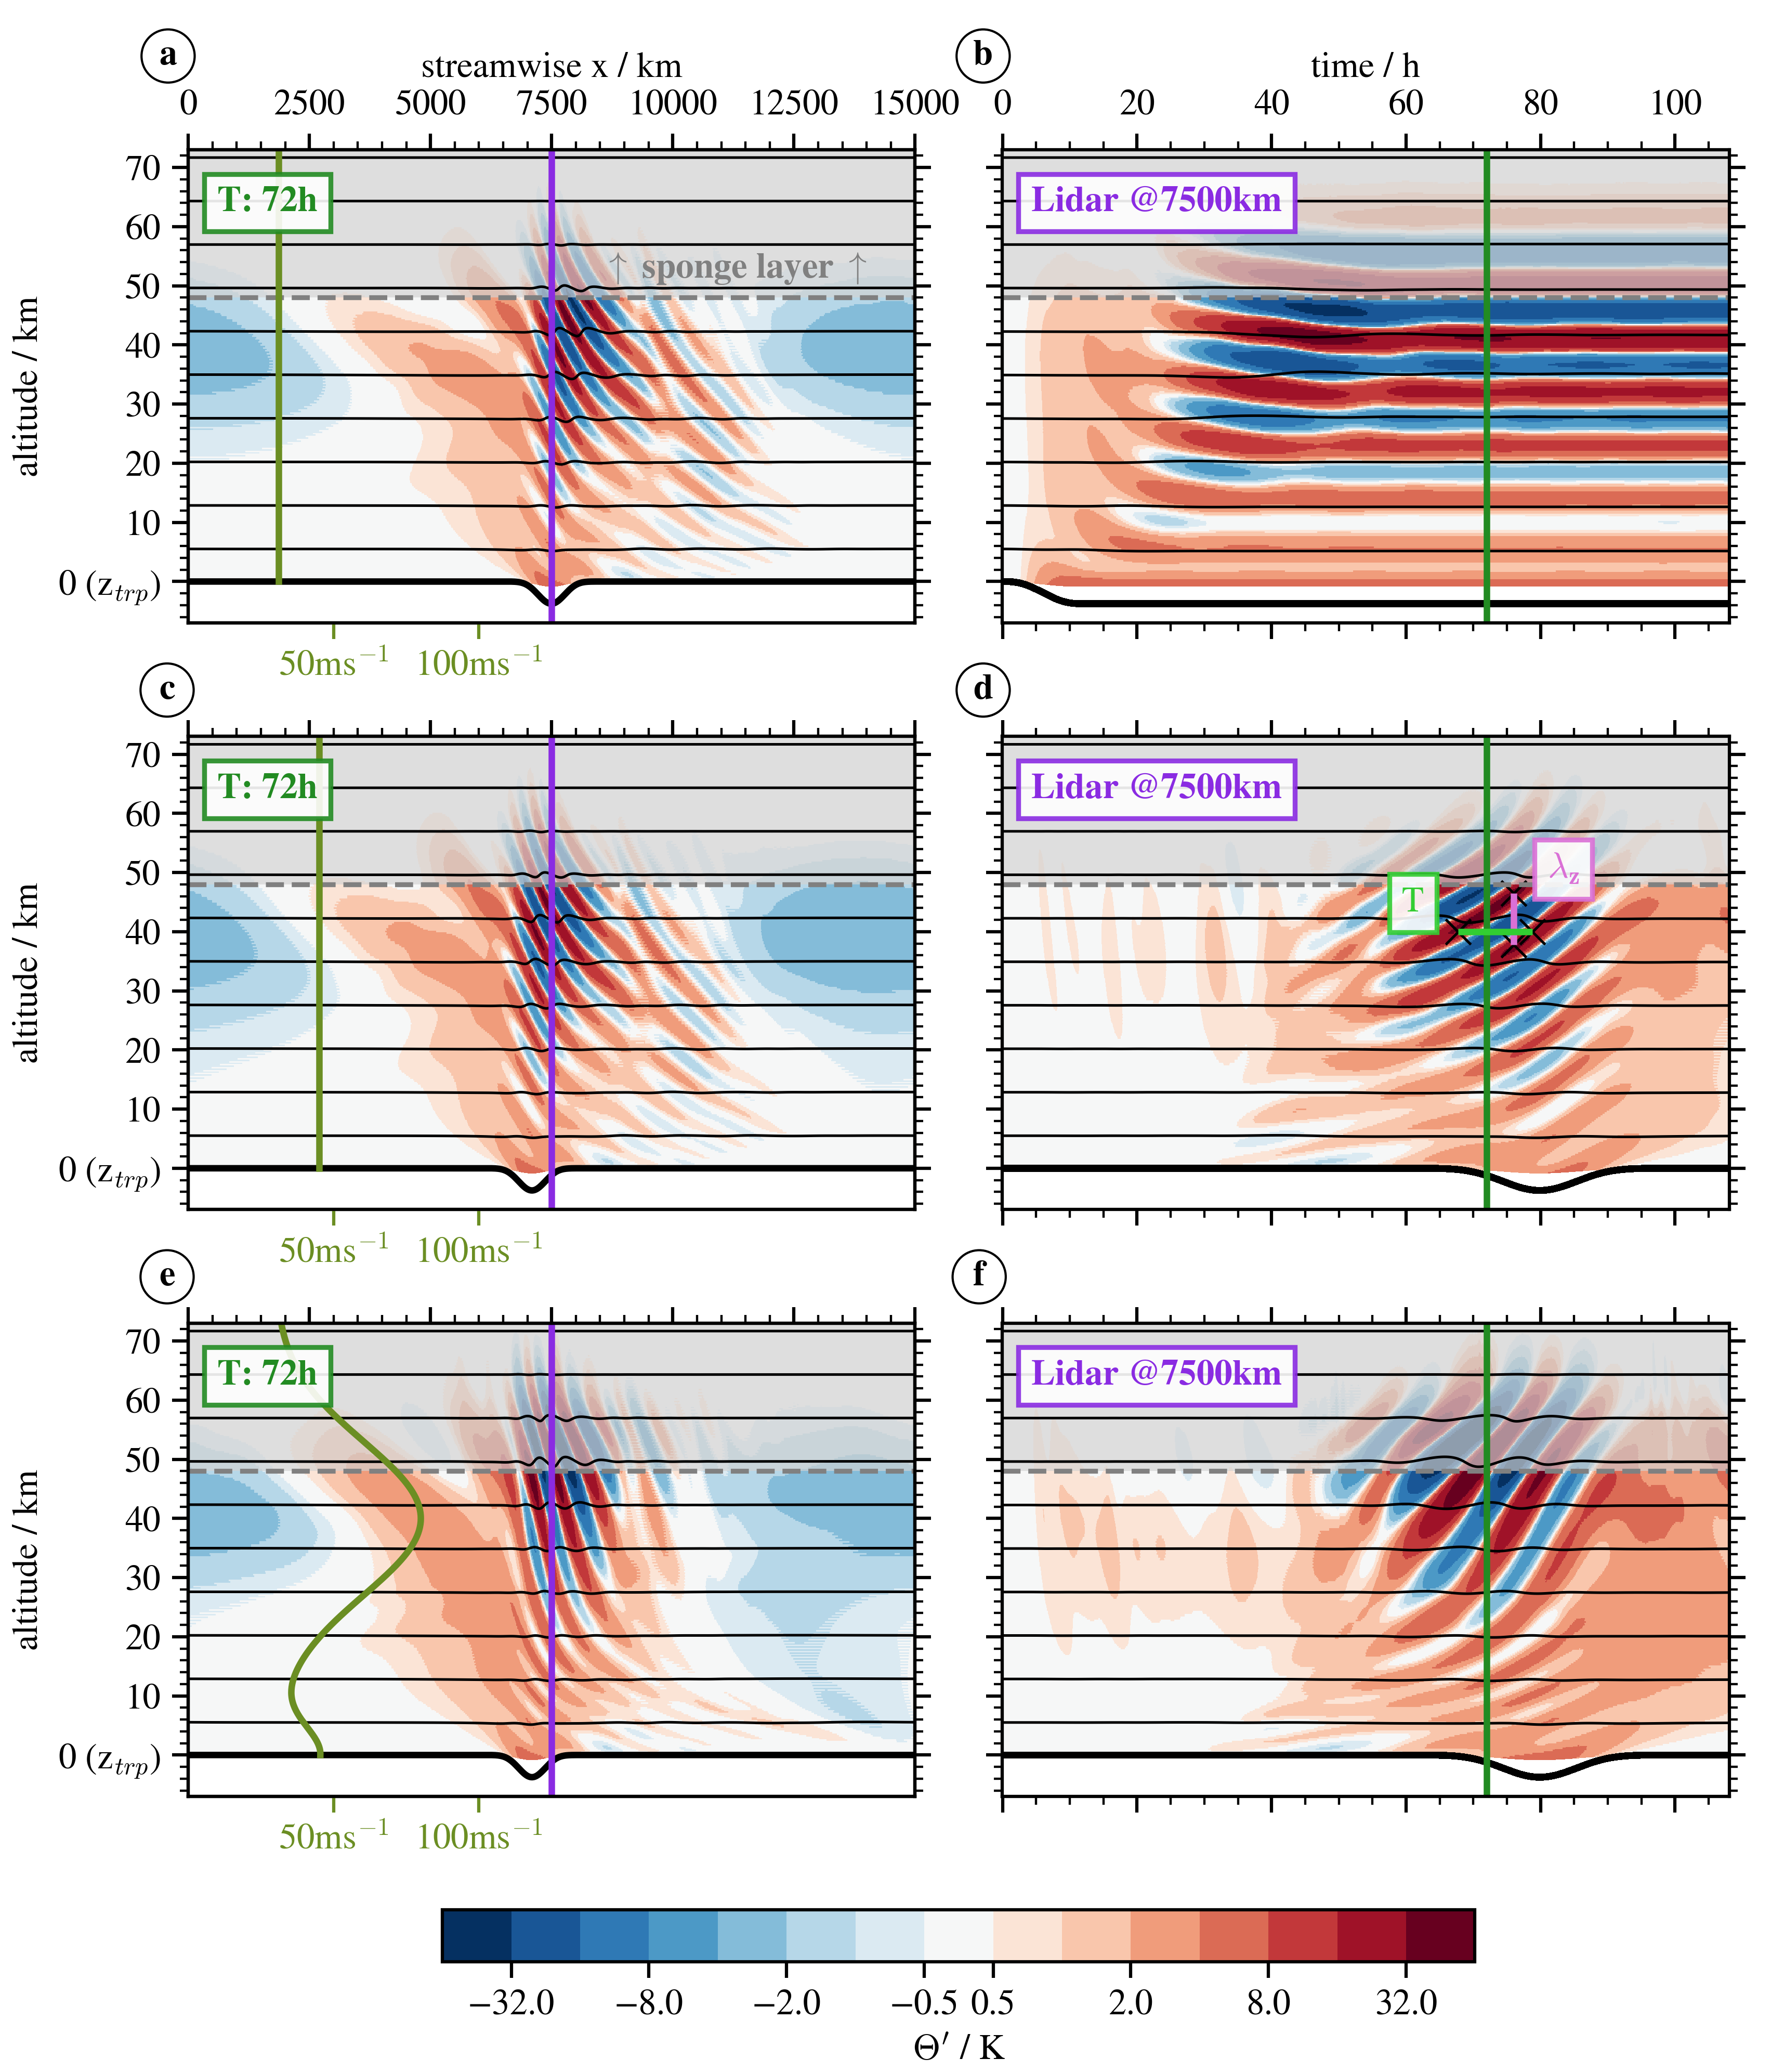
\includegraphics[width=0.99\textwidth]{figures_lidar/lidana_th.png}
    \caption{Shown are vertical cross-sections (a,c,e) after $t$=\SI{72}{\hour} with vertical wind profiles in green and vertical time series (b,d,f) at the outlined position for three different simulations. The first simulation (a,b) features a stationary obstacle at the lower boundary and a constant wind profile. In the second simulation (c,d) the trough moves to the right with a constant speed $c_{source}$=\SI{13.88}{\meter \per \second} and the wind is increased by the same amount. The last simulation (e,f) represents the reference simulation of the sensitivity analysis in section \ref{sec:resultsQ3D} with a more realistic stratospheric winter time wind profile. The assessment of $\lambda_z$ and period $T$ from the vertical time series is labeled in (d), two consecutive $\lambda_x$ are labeled in (c). Contour lines represent constant potential temperature and the amplitude of the lower boundary is scaled by a factor of 5.}
    \label{fig:lidar_sim}
\end{figure*}

Within the framework of this work, let us stay with the last explanation and think through the GW characterization for the simplified case of a constant wind profile shown in Figure \ref{fig:lidar_sim}c and \ref{fig:lidar_sim}d. To recap, a constant stratification with $N=\SI{0.02}{\per \second}$ was used for all simulations starting at the tropopause simplifying the dispersion relation for Boussinesq flows to

\begin{equation}
    \hat{w}^2 = \frac{N^2k^2}{k^2+m^2} = Ncos(\phi).
    \label{equ_lid:dispersion}
    % observed waves obey a dispersion relation for internal Boussinesq
    % Alhough variations in density are the very essence of buoyancy, they are neglected everywhere in the Boussinesq equations “except in so far as they modify the action of gravity” (Rayleigh, 1916), i.e., the density is assumed to be constant except in the buoyancy force
    % by applying a peak finding algorith to the vertical profile and additionally a time span $T$ applying the same algorithm along the time axis
\end{equation}

As labeled in Figure \ref{fig:lidar_sim}d, the vertical distance between troughs or ridges in the vertical time series yields the vertical wavelength $\lambda_z=\SI{9.25}{\kilo \meter}$ and wavenumber $m$, the horizontal distance at \SI{40}{\kilo \meter} provides a period $T=\SI{13.92}{\hour}$ and ground-based frequency $\omega$. How can this frequency be interpreted? If we assume a fully developed stationary wave field above the depression that propagates with its source, the tilt of the phase lines within the lidar observation depends on the propagation speed of the GW source and the horizontal wavelength $\lambda_x$. Thus, a constant propagation speed $c_{source}$=\SI{13.88}{\meter \per \second} leads to $\lambda_x = T \cdot c_{source}$= \SI{695}{\kilo \meter}, which is in the range of wavelengths labeled in the vertical cross-section(Figure\ref{fig:lidar_sim}c) at the same height with $\lambda_x$=\SI{525}{\kilo \meter} - \SI{712}{\kilo \meter}. The ratio of $\lambda_x$ and $\lambda_z$ provides 

\begin{equation}
    \phi = \tan^{-1}(\frac{\lambda_x}{\lambda_z}) 
    \label{equ_lid:phi}
\end{equation}

and 

\begin{equation}
    c_{px} = \frac{N}{k} cos(\phi), \qquad c_{pz} = \frac{N}{m} cos(\phi)
    \label{equ_lid:cp}
\end{equation}


vertical waIn a next step,

Continueing the analysis with this satisfying result....

angle phi

pahse speeds
group speeds

check slides






- For stationary mountain waves the . For a transient/propagating GW source this results in $c_{px}=-u+c_{source}$ with $c_{px}$ balancing the wind speed forcing described in section \ref{sec:resultsQ3D}.



Extend conclusions of \textcite{dornbrack_interpretation_2017}.

% The slope of the phase lines in a horizontal time series taken at fixed altitude is equal to cPx. from Dörnbrack -> not true for propagating source

% Summarizing the assumptions involved so far if we would like to retrieve wave properties from the virtual time series observations as presented in Figure 6:

% \begin{equation}
%     \lambda_z = \frac{2*\Pi}{m} 
% \end{equation}



% Assuming \textcite{dornbrack_interpretation_2017}., the recorded period $T = 2π/ω$ can be used to obtain an estimate of the ground-based frequency ω. In such a case, the slope of the phase lines gives the vertical phase speed cPz = ± λz/T and the propagation directions of the wave phases and of the wave packet, respectively. Using an estimate of the background stratification N, the phase angle φ can be estimated from Equation (8) and k can be computed. Technically, the Equations (12) and (13) can now be employed to derive the components of the group velocity cgx and cgz from the known values of k, m, and φ. Summarizing the assumpti

show for constant wind and idealized stratospheric winter profile

In the thorough descripition of 


As usual, the vertical wavelength in the  be derived from the Lidar observation with


\begin{equation}
\begin{aligned}
    c_{px} = \frac{N}{k} cos(\phi), \qquad c_{pz} = \frac{N}{m} cos(\phi)
    % \label{equ:momEqu}
\end{aligned}
\end{equation}



% First of all, there have to be sufficiently large tropospheric winds perpendicular to the mountain ridge for excitation of MWs (e.g., Bramberger et al., 2017; Dörnbrack et al., 1999; Kaifler, Kaifler, et  al.,  2015). In addition, Dörnbrack et  al.  (1999) report that good excitation conditions prevail when the wind turns no more than 30° within the first 30 km. Monthly mean wind speeds in ERA5 data are at about 𝐴𝐴 15 ms−1 at surface level (500 m) at all times. The wind rotation within the first 30 km is <30° during the months from March to October with a surface level forcing between 240° and 280°. Thus, in the climatological mean MWs are excited and able to propagate deep into the middle atmosphere in the winter months. A strong wind rotation within the first 30 km of about 60° can only be observed in July 2020. At this time, we also find reduced GW energies at all altitude regions (see Figure 6). For upward propagation, the wind speed in the direction of wave propagation must not become zero as this would lead to wave breaking (Lindzen,  1981). Moreover, for deep vertical propagation, the MWs should not encounter turning levels where the intrinsic frequency approaches the buoyancy frequency (e.g., Schoeberl, 1985). These conditions occur in the core of the PNJ and filter horizontally short MWs or lead to evanescent modes tunneling through the PNJ (e.g., Mixa et al., 2021). Another obstacle for MWs is the stratospheric wind minimum where the waves' 𝐴𝐴𝐴𝐴′-amplitude may become equal to the horizontal wind speed causing wave breaking. This wind minimum can act as a valve for vertically propagating MWs (Kruse et al., 2016). Figure 10 reveals that low wind speeds at ∼25 km altitude occur from March to May. In the winter months, with positive temperature gradients (Figure 2) and large horizontal wind speeds (Figure 10) up to 50 km, generally good vertical propagation conditions can be expected. Above, shear instabilities and unstable lapse rates lead to wave dissipation. On the other hand, the mesosphere is the favorable region for the generation of secondary gravity waves (Heale et al., 2020; Kogure et al., 2020; Vadas & Becker, 2019; Vadas et al., 2018). Large contributions of apparently up- and downward propagating waves and reduced contributions of stationary waves (see Table 3) at mesospheric altitudes might indicate their existence above Río Grande.



\section{CORAL observations of NOGWs from a transient source}
\label{sec:lidOb-coral}

% In addition, the latitudinal position of the PNJ over the Southern Andes can change significantly over the course of several weeks. As the PNJ is responsible for the refraction of waves toward larger vertical wavelengths, this mechanism in combination with a fixed 𝐴𝐴𝐴𝐴cut might also affect the derivation of potential energies.

This section provides a short introduction to an interesting Lidar observation of the Compact Autonomous Rayleigh Lidar (CORAL) at the southern tip of South America in Rio Grande, Argentina. 

Short description of CORAL...

Discussion of plots:

- GWs in upper atmosphere + background wind!!

- lower plot: Forcing conditions at surface 

- eventually wind profile over time could be helpful with interpretation

- state that vertical time series would look quite similar to observations - angle of idealized simulation for realistic wind profile -> approximately 20km / 12h 


- second case: time of observation could fit to tropopause fold... waves develope into the lee of the fold... but wind direction turns towards NW might be another explanation.

\textcite{kaifler_compact_2021} provide a more extensive summary on CORAL's setup and observation, 

focus on observation from July 28th, 2018 showing upwards tilted lines of constant phase between 

\begin{figure*}[tbp]
    \centering
    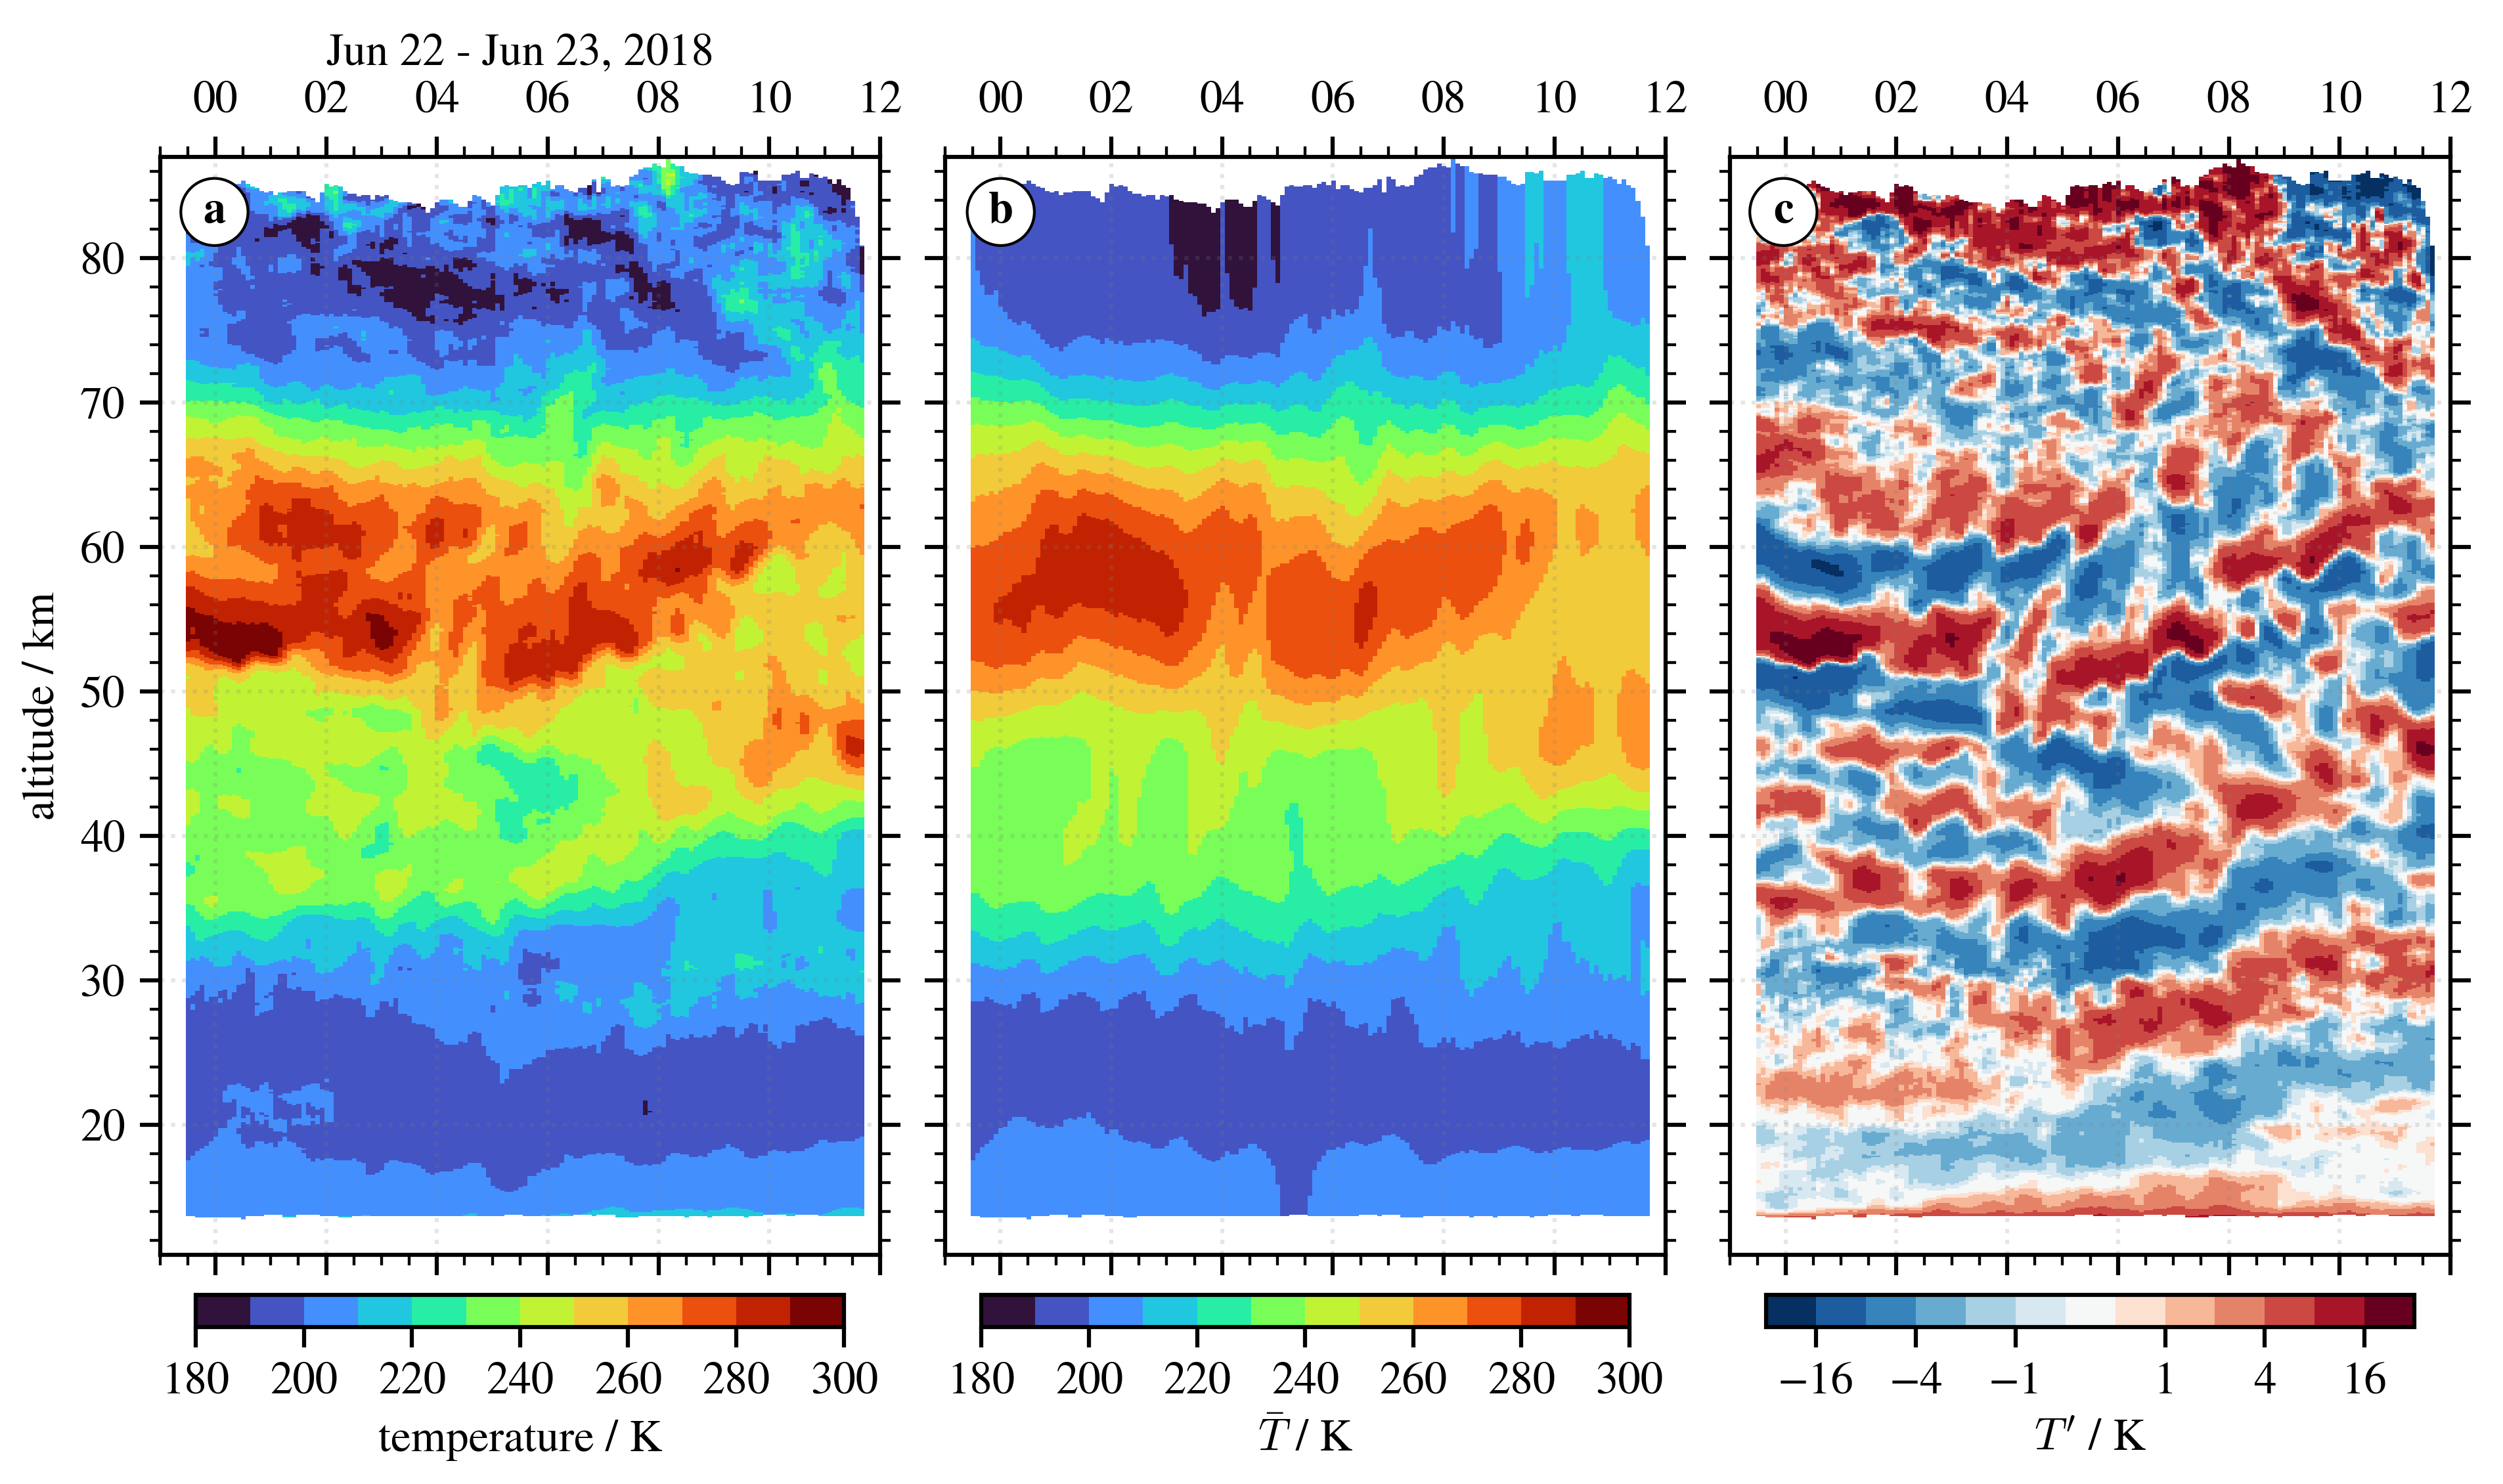
\includegraphics[width=0.99\textwidth]{figures_lidar/coral_event_20180622.png}
    \caption{Vertical cross sections at 40km above the tropopause for five simulations with horizontal and meridional shear in a barotropic environment. Shown are $\theta$', $\lambda_x$ and $\lambda_y$ at 72h into the simulation. Dominant zonal and meridional wavelengths for each grid point are determined from wavelet analysis.}
    % \label{fig:waveletAna_dudy}
\end{figure*}


\begin{figure*}[tbp]
    \centering
    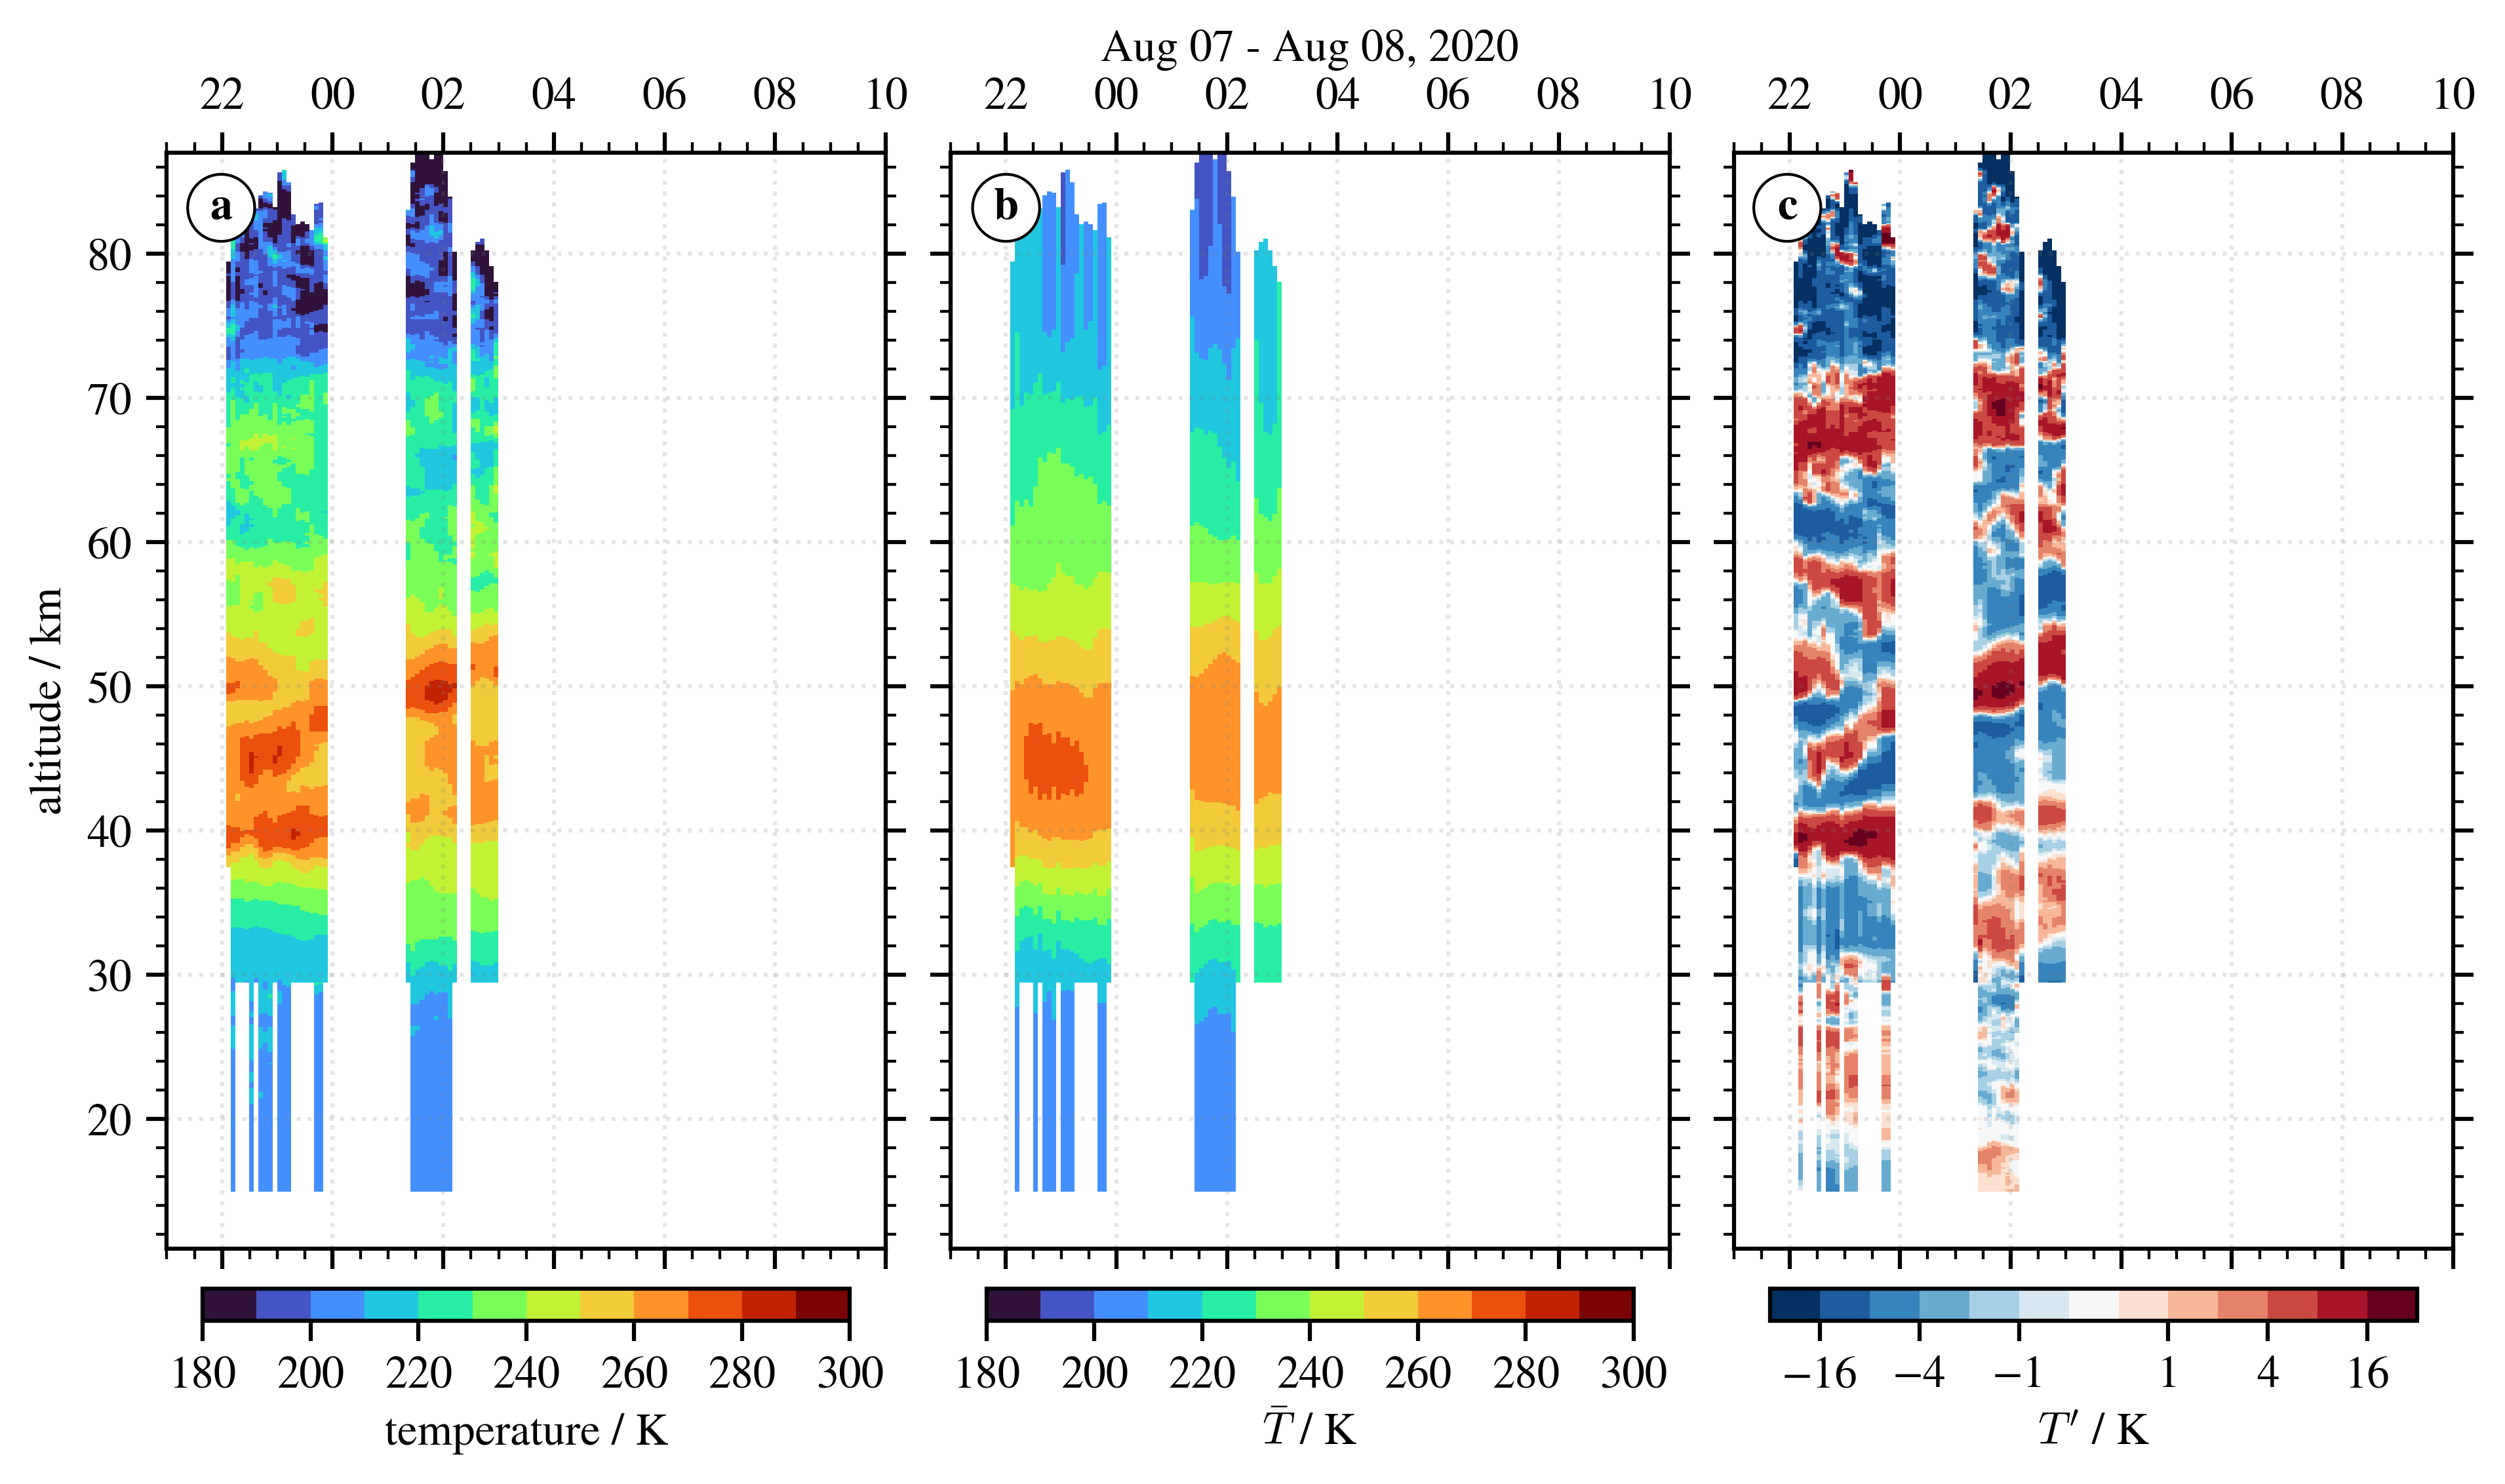
\includegraphics[width=0.99\textwidth]{figures_lidar/coral_event_20200807.png}
    \caption{}
    % \label{fig:waveletAna_dudy}
\end{figure*}


\begin{figure*}[tbp]
    \centering
    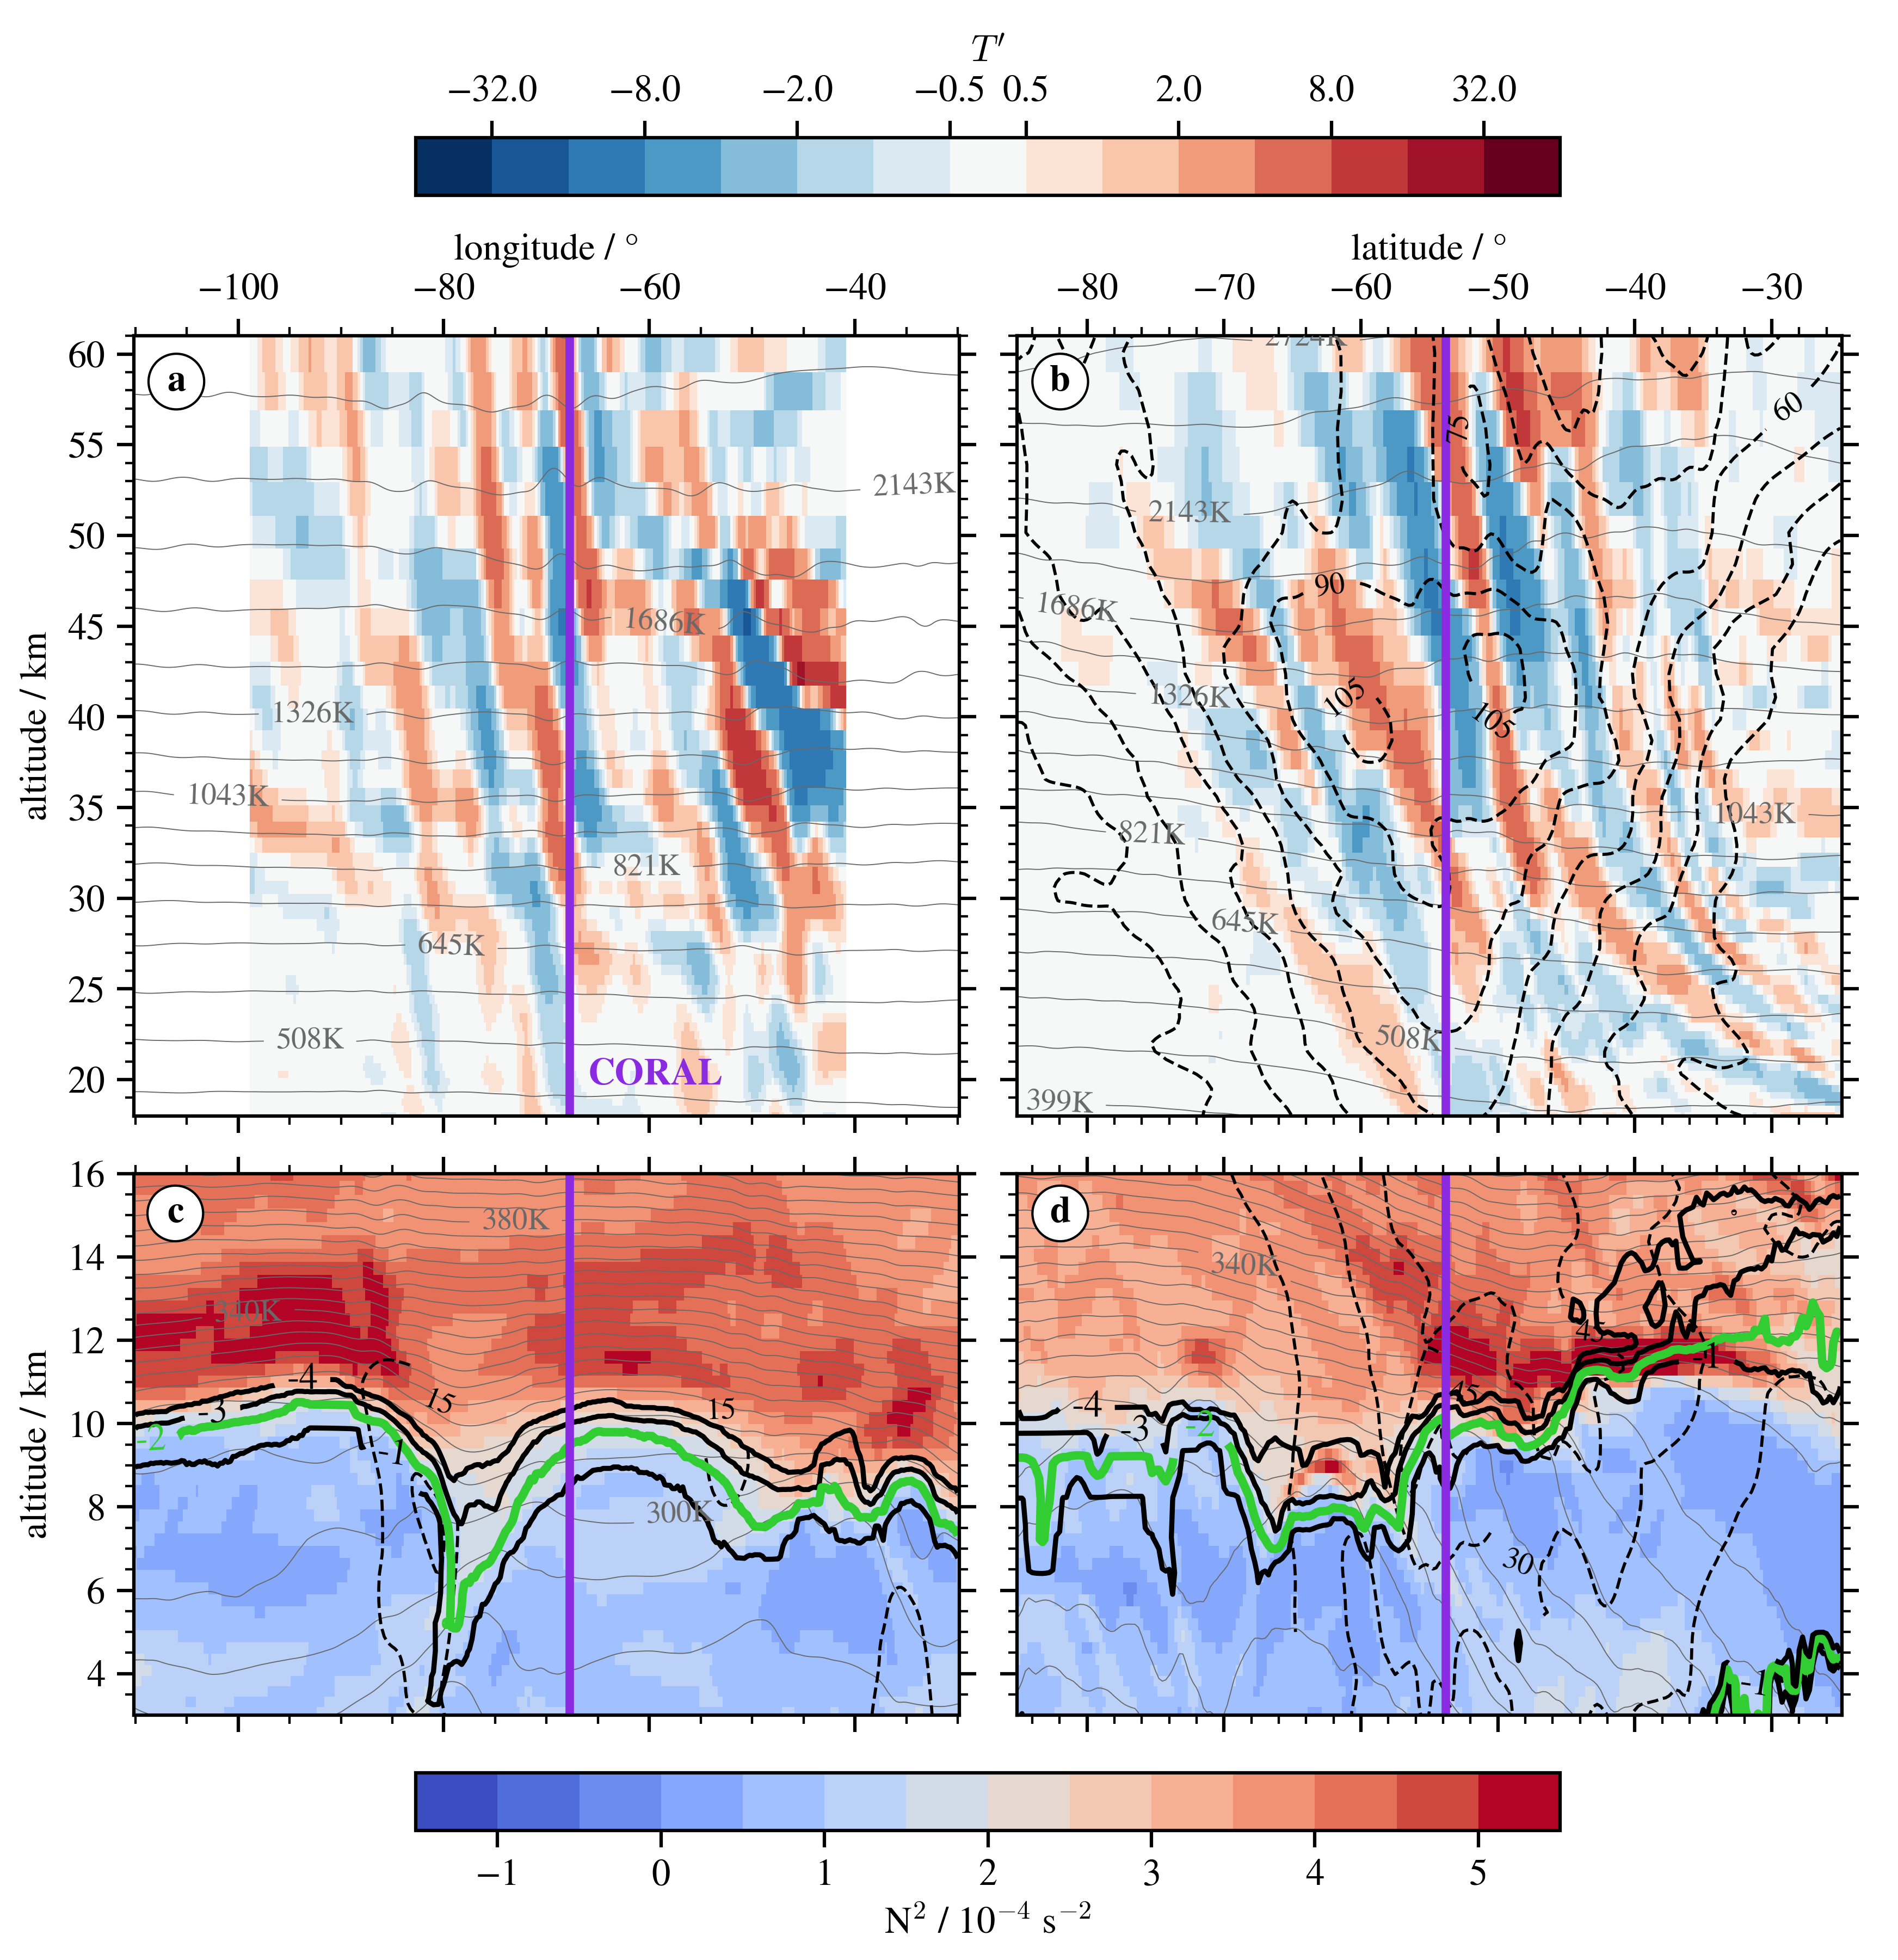
\includegraphics[width=0.99\textwidth]{figures_lidar/era5_trop_strat_2.png}
    \caption{Vertical cross sections of the stratosphere along 57.75°S (a) and 67°E (b)}
    % \label{fig:waveletAna_dudy}
\end{figure*}
